%%%%%%%% ICML 2025 EXAMPLE LATEX SUBMISSION FILE %%%%%%%%%%%%%%%%%

\documentclass{article}
\usepackage{tikz}
\usepackage{tikz}
\usetikzlibrary{shapes.geometric, arrows, positioning}

\tikzstyle{layer} = [rectangle, rounded corners, minimum width=3.5cm, minimum height=1cm, text centered, draw=black, fill=blue!20]
\tikzstyle{arrow} = [thick,->,>=stealth]

% Recommended, but optional, packages for figures and better typesetting:
\usepackage{microtype}
\usepackage{graphicx}
\usepackage{subfigure}
\usepackage{booktabs} % for professional tables



% hyperref makes hyperlinks in the resulting PDF.
% If your build breaks (sometimes temporarily if a hyperlink spans a page)
% please comment out the following usepackage line and replace
% \usepackage{icml2025} with \usepackage[nohyperref]{icml2025} above.
\usepackage{hyperref}


% Attempt to make hyperref and algorithmic work together better:
\newcommand{\theHalgorithm}{\arabic{algorithm}}

% Use the following line for the initial blind version submitted for review:
% \usepackage{icml2025}

% If accepted, instead use the following line for the camera-ready submission:
\usepackage[accepted]{icml2025}

% For theorems and such
\usepackage{amsmath}
\usepackage{amssymb}
\usepackage{mathtools}
\usepackage{amsthm}

% if you use cleveref..
\usepackage[capitalize,noabbrev]{cleveref}

%%%%%%%%%%%%%%%%%%%%%%%%%%%%%%%%
% THEOREMS
%%%%%%%%%%%%%%%%%%%%%%%%%%%%%%%%
\theoremstyle{plain}
\newtheorem{theorem}{Theorem}[section]
\newtheorem{proposition}[theorem]{Proposition}
\newtheorem{lemma}[theorem]{Lemma}
\newtheorem{corollary}[theorem]{Corollary}
\theoremstyle{definition}
\newtheorem{definition}[theorem]{Definition}
\newtheorem{assumption}[theorem]{Assumption}
\theoremstyle{remark}
\newtheorem{remark}[theorem]{Remark}

% Todonotes is useful during development; simply uncomment the next line
%    and comment out the line below the next line to turn off comments
%\usepackage[disable,textsize=tiny]{todonotes}
\usepackage[textsize=tiny]{todonotes}


% The \icmltitle you define below is probably too long as a header.
% Therefore, a short form for the running title is supplied here:
\icmltitlerunning{Submission and Formatting Instructions for ICML 2025}

\begin{document}

\twocolumn[
\icmltitle{Zero-Shot Forecasting and Neural Operators \\ Master Lab
}

% It is OKAY to include author information, even for blind
% submissions: the style file will automatically remove it for you
% unless you've provided the [accepted] option to the icml2025
% package.

% List of affiliations: The first argument should be a (short)
% identifier you will use later to specify author affiliations
% Academic affiliations should list Department, University, City, Region, Country
% Industry affiliations should list Company, City, Region, Country

% You can specify symbols, otherwise they are numbered in order.
% Ideally, you should not use this facility. Affiliations will be numbered
% in order of appearance and this is the preferred way.
\icmlsetsymbol{equal}{*}

\begin{icmlauthorlist}
\icmlauthor{Arwin ---}{equal,yyy}
\icmlauthor{Jan Hardtke}{equal,yyy,comp}
\icmlauthor{Nadia Gharbi}{comp}

\end{icmlauthorlist}

\icmlaffiliation{yyy}{Department of XXX, University of YYY, Location, Country}
\icmlaffiliation{comp}{Company Name, Location, Country}

\icmlcorrespondingauthor{Firstname1 Lastname1}{first1.last1@xxx.edu}
\icmlcorrespondingauthor{Firstname2 Lastname2}{first2.last2@www.uk}

% You may provide any keywords that you
% find helpful for describing your paper; these are used to populate
% the "keywords" metadata in the PDF but will not be shown in the document
\icmlkeywords{Machine Learning, ICML}

\vskip 0.3in
]

% this must go after the closing bracket ] following \twocolumn[ ...

% This command actually creates the footnote in the first column
% listing the affiliations and the copyright notice.
% The command takes one argument, which is text to display at the start of the footnote.
% The \icmlEqualContribution command is standard text for equal contribution.
% Remove it (just {}) if you do not need this facility.

%\printAffiliationsAndNotice{}  % leave blank if no need to mention equal contribution
\printAffiliationsAndNotice{\icmlEqualContribution} % otherwise use the standard text.

\begin{abstract}
A
\end{abstract}

\section{Structure}

- abstract \\
- a brief introduction (Nadia) \\ 
- a discussion of related work (Decoder Only, Statistical models like ARIMA, (briefly FIM-l and DeepONet with reference to chapter conceptual aspects) ... do more research...) (Nadia) \\ 
- An explanation of the main conceptual aspects (e.g. DeepONets, random function generation and maybe zero-shot learning) is expected. (Arwin) \\ 
- In an experimental section, give details for reproducibility of your work (e.g. hyperparameters, training objectives, hardware, runtime...). (Jan) \\ 
- A results section could include a description of the tasks and your findings (use tables and figures to present your results). \\
- Finish the report with a short concluding section.

- Note that you are encouraged to further improve and explore the models for each task! (Jan)

\section{Electronic Submission}
\label{submission}

Submission to ICML 2025 will be entirely electronic, via a web site
(not email). Information about the submission process and \LaTeX\ templates
are available on the conference web site at:
\begin{center}
\textbf{\texttt{http://icml.cc/}}
\end{center}

The guidelines below will be enforced for initial submissions and
camera-ready copies. Here is a brief summary:
\begin{itemize}
\item Submissions must be in PDF\@. 
\item If your paper has appendices, submit the appendix together with the main body and the references \textbf{as a single file}. Reviewers will not look for appendices as a separate PDF file. So if you submit such an extra file, reviewers will very likely miss it.
\item Page limit: The main body of the paper has to be fitted to 8 pages, excluding references and appendices; the space for the latter two is not limited in pages, but the total file size may not exceed 10MB. For the final version of the paper, authors can add one extra page to the main body.
\item \textbf{Do not include author information or acknowledgements} in your
    initial submission.
\item Your paper should be in \textbf{10 point Times font}.
\item Make sure your PDF file only uses Type-1 fonts.
\item Place figure captions \emph{under} the figure (and omit titles from inside
    the graphic file itself). Place table captions \emph{over} the table.
\item References must include page numbers whenever possible and be as complete
    as possible. Place multiple citations in chronological order.
\item Do not alter the style template; in particular, do not compress the paper
    format by reducing the vertical spaces.
\item Keep your abstract brief and self-contained, one paragraph and roughly
    4--6 sentences. Gross violations will require correction at the
    camera-ready phase. The title should have content words capitalized.
\end{itemize}

\subsection{Submitting Papers}

\textbf{Anonymous Submission:} ICML uses double-blind review: no identifying
author information may appear on the title page or in the paper
itself. \cref{author info} gives further details.

\medskip

Authors must provide their manuscripts in \textbf{PDF} format.
Furthermore, please make sure that files contain only embedded Type-1 fonts
(e.g.,~using the program \texttt{pdffonts} in linux or using
File/DocumentProperties/Fonts in Acrobat). Other fonts (like Type-3)
might come from graphics files imported into the document.

Authors using \textbf{Word} must convert their document to PDF\@. Most
of the latest versions of Word have the facility to do this
automatically. Submissions will not be accepted in Word format or any
format other than PDF\@. Really. We're not joking. Don't send Word.

Those who use \textbf{\LaTeX} should avoid including Type-3 fonts.
Those using \texttt{latex} and \texttt{dvips} may need the following
two commands:

{\footnotesize
\begin{verbatim}
dvips -Ppdf -tletter -G0 -o paper.ps paper.dvi
ps2pdf paper.ps
\end{verbatim}}
It is a zero following the ``-G'', which tells dvips to use
the config.pdf file. Newer \TeX\ distributions don't always need this
option.

Using \texttt{pdflatex} rather than \texttt{latex}, often gives better
results. This program avoids the Type-3 font problem, and supports more
advanced features in the \texttt{microtype} package.

\textbf{Graphics files} should be a reasonable size, and included from
an appropriate format. Use vector formats (.eps/.pdf) for plots,
lossless bitmap formats (.png) for raster graphics with sharp lines, and
jpeg for photo-like images.

The style file uses the \texttt{hyperref} package to make clickable
links in documents. If this causes problems for you, add
\texttt{nohyperref} as one of the options to the \texttt{icml2025}
usepackage statement.


\subsection{Submitting Final Camera-Ready Copy}

The final versions of papers accepted for publication should follow the
same format and naming convention as initial submissions, except that
author information (names and affiliations) should be given. See
\cref{final author} for formatting instructions.

The footnote, ``Preliminary work. Under review by the International
Conference on Machine Learning (ICML). Do not distribute.'' must be
modified to ``\textit{Proceedings of the
$\mathit{42}^{nd}$ International Conference on Machine Learning},
Vancouver, Canada, PMLR 267, 2025.
Copyright 2025 by the author(s).''

For those using the \textbf{\LaTeX} style file, this change (and others) is
handled automatically by simply changing
$\mathtt{\backslash usepackage\{icml2025\}}$ to
$$\mathtt{\backslash usepackage[accepted]\{icml2025\}}$$
Authors using \textbf{Word} must edit the
footnote on the first page of the document themselves.

Camera-ready copies should have the title of the paper as running head
on each page except the first one. The running title consists of a
single line centered above a horizontal rule which is $1$~point thick.
The running head should be centered, bold and in $9$~point type. The
rule should be $10$~points above the main text. For those using the
\textbf{\LaTeX} style file, the original title is automatically set as running
head using the \texttt{fancyhdr} package which is included in the ICML
2025 style file package. In case that the original title exceeds the
size restrictions, a shorter form can be supplied by using

\verb|\icmltitlerunning{...}|

just before $\mathtt{\backslash begin\{document\}}$.
Authors using \textbf{Word} must edit the header of the document themselves.

\section{Format of the Paper}

All submissions must follow the specified format.

\subsection{Dimensions}




The text of the paper should be formatted in two columns, with an
overall width of 6.75~inches, height of 9.0~inches, and 0.25~inches
between the columns. The left margin should be 0.75~inches and the top
margin 1.0~inch (2.54~cm). The right and bottom margins will depend on
whether you print on US letter or A4 paper, but all final versions
must be produced for US letter size.
Do not write anything on the margins.

The paper body should be set in 10~point type with a vertical spacing
of 11~points. Please use Times typeface throughout the text.

\subsection{Title}

The paper title should be set in 14~point bold type and centered
between two horizontal rules that are 1~point thick, with 1.0~inch
between the top rule and the top edge of the page. Capitalize the
first letter of content words and put the rest of the title in lower
case.

\subsection{Author Information for Submission}
\label{author info}

ICML uses double-blind review, so author information must not appear. If
you are using \LaTeX\/ and the \texttt{icml2025.sty} file, use
\verb+\icmlauthor{...}+ to specify authors and \verb+\icmlaffiliation{...}+ to specify affiliations. (Read the TeX code used to produce this document for an example usage.) The author information
will not be printed unless \texttt{accepted} is passed as an argument to the
style file.
Submissions that include the author information will not
be reviewed.

\subsubsection{Self-Citations}

If you are citing published papers for which you are an author, refer
to yourself in the third person. In particular, do not use phrases
that reveal your identity (e.g., ``in previous work, we
have shown \ldots'').

Do not anonymize citations in the reference section. The only exception are manuscripts that are
not yet published (e.g., under submission). If you choose to refer to
such unpublished manuscripts, anonymized copies have
to be submitted
as Supplementary Material via OpenReview\@. However, keep in mind that an ICML
paper should be self contained and should contain sufficient detail
for the reviewers to evaluate the work. In particular, reviewers are
not required to look at the Supplementary Material when writing their
review (they are not required to look at more than the first $8$ pages of the submitted document).

\subsubsection{Camera-Ready Author Information}
\label{final author}

If a paper is accepted, a final camera-ready copy must be prepared.
%
For camera-ready papers, author information should start 0.3~inches below the
bottom rule surrounding the title. The authors' names should appear in 10~point
bold type, in a row, separated by white space, and centered. Author names should
not be broken across lines. Unbolded superscripted numbers, starting 1, should
be used to refer to affiliations.

Affiliations should be numbered in the order of appearance. A single footnote
block of text should be used to list all the affiliations. (Academic
affiliations should list Department, University, City, State/Region, Country.
Similarly for industrial affiliations.)

Each distinct affiliations should be listed once. If an author has multiple
affiliations, multiple superscripts should be placed after the name, separated
by thin spaces. If the authors would like to highlight equal contribution by
multiple first authors, those authors should have an asterisk placed after their
name in superscript, and the term ``\textsuperscript{*}Equal contribution"
should be placed in the footnote block ahead of the list of affiliations. A
list of corresponding authors and their emails (in the format Full Name
\textless{}email@domain.com\textgreater{}) can follow the list of affiliations.
Ideally only one or two names should be listed.

A sample file with author names is included in the ICML2025 style file
package. Turn on the \texttt{[accepted]} option to the stylefile to
see the names rendered. All of the guidelines above are implemented
by the \LaTeX\ style file.

\subsection{Abstract}

The paper abstract should begin in the left column, 0.4~inches below the final
address. The heading `Abstract' should be centered, bold, and in 11~point type.
The abstract body should use 10~point type, with a vertical spacing of
11~points, and should be indented 0.25~inches more than normal on left-hand and
right-hand margins. Insert 0.4~inches of blank space after the body. Keep your
abstract brief and self-contained, limiting it to one paragraph and roughly 4--6
sentences. Gross violations will require correction at the camera-ready phase.

\subsection{Partitioning the Text}

You should organize your paper into sections and paragraphs to help
readers place a structure on the material and understand its
contributions.

\subsubsection{Sections and Subsections}

Section headings should be numbered, flush left, and set in 11~pt bold
type with the content words capitalized. Leave 0.25~inches of space
before the heading and 0.15~inches after the heading.

Similarly, subsection headings should be numbered, flush left, and set
in 10~pt bold type with the content words capitalized. Leave
0.2~inches of space before the heading and 0.13~inches afterward.

Finally, subsubsection headings should be numbered, flush left, and
set in 10~pt small caps with the content words capitalized. Leave
0.18~inches of space before the heading and 0.1~inches after the
heading.

Please use no more than three levels of headings.

\subsubsection{Paragraphs and Footnotes}

Within each section or subsection, you should further partition the
paper into paragraphs. Do not indent the first line of a given
paragraph, but insert a blank line between succeeding ones.

You can use footnotes\footnote{Footnotes
should be complete sentences.} to provide readers with additional
information about a topic without interrupting the flow of the paper.
Indicate footnotes with a number in the text where the point is most
relevant. Place the footnote in 9~point type at the bottom of the
column in which it appears. Precede the first footnote in a column
with a horizontal rule of 0.8~inches.\footnote{Multiple footnotes can
appear in each column, in the same order as they appear in the text,
but spread them across columns and pages if possible.}

\begin{figure}[ht]
\vskip 0.2in
\begin{center}
\centerline{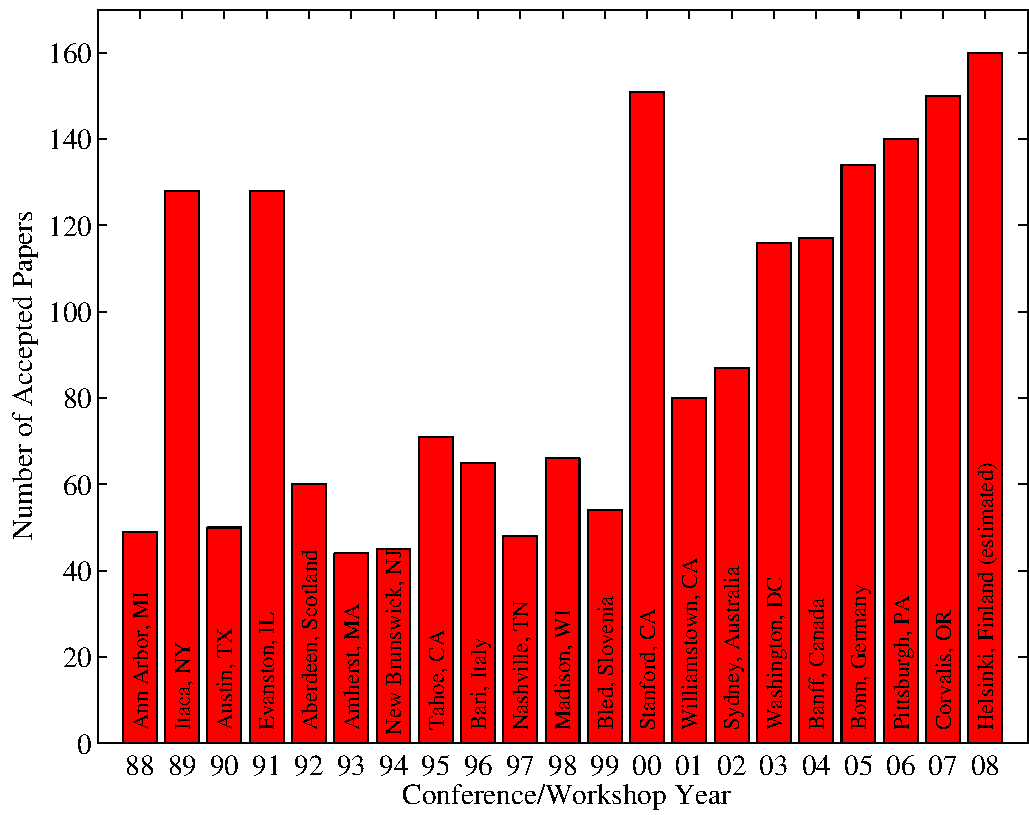
\includegraphics[width=\columnwidth]{icml_numpapers}}
\caption{Historical locations and number of accepted papers for International
Machine Learning Conferences (ICML 1993 -- ICML 2008) and International
Workshops on Machine Learning (ML 1988 -- ML 1992). At the time this figure was
produced, the number of accepted papers for ICML 2008 was unknown and instead
estimated.}
\label{icml-historical}
\end{center}
\vskip -0.2in
\end{figure}

\subsection{Figures}

You may want to include figures in the paper to illustrate
your approach and results. Such artwork should be centered,
legible, and separated from the text. Lines should be dark and at
least 0.5~points thick for purposes of reproduction, and text should
not appear on a gray background.

Label all distinct components of each figure. If the figure takes the
form of a graph, then give a name for each axis and include a legend
that briefly describes each curve. Do not include a title inside the
figure; instead, the caption should serve this function.

Number figures sequentially, placing the figure number and caption
\emph{after} the graphics, with at least 0.1~inches of space before
the caption and 0.1~inches after it, as in
\cref{icml-historical}. The figure caption should be set in
9~point type and centered unless it runs two or more lines, in which
case it should be flush left. You may float figures to the top or
bottom of a column, and you may set wide figures across both columns
(use the environment \texttt{figure*} in \LaTeX). Always place
two-column figures at the top or bottom of the page.

\subsection{Algorithms}

If you are using \LaTeX, please use the ``algorithm'' and ``algorithmic''
environments to format pseudocode. These require
the corresponding stylefiles, algorithm.sty and
algorithmic.sty, which are supplied with this package.
\cref{alg:example} shows an example.

\begin{algorithm}[tb]
   \caption{Bubble Sort}
   \label{alg:example}
\begin{algorithmic}
   \STATE {\bfseries Input:} data $x_i$, size $m$
   \REPEAT
   \STATE Initialize $noChange = true$.
   \FOR{$i=1$ {\bfseries to} $m-1$}
   \IF{$x_i > x_{i+1}$}
   \STATE Swap $x_i$ and $x_{i+1}$
   \STATE $noChange = false$
   \ENDIF
   \ENDFOR
   \UNTIL{$noChange$ is $true$}
\end{algorithmic}
\end{algorithm}

\subsection{Tables}

You may also want to include tables that summarize material. Like
figures, these should be centered, legible, and numbered consecutively.
However, place the title \emph{above} the table with at least
0.1~inches of space before the title and the same after it, as in
\cref{sample-table}. The table title should be set in 9~point
type and centered unless it runs two or more lines, in which case it
should be flush left.

% Note use of \abovespace and \belowspace to get reasonable spacing
% above and below tabular lines.

\begin{table}[t]
\caption{Classification accuracies for naive Bayes and flexible
Bayes on various data sets.}
\label{sample-table}
\vskip 0.15in
\begin{center}
\begin{small}
\begin{sc}
\begin{tabular}{lcccr}
\toprule
Data set & Naive & Flexible & Better? \\
\midrule
Breast    & 95.9$\pm$ 0.2& 96.7$\pm$ 0.2& $\surd$ \\
Cleveland & 83.3$\pm$ 0.6& 80.0$\pm$ 0.6& $\times$\\
Glass2    & 61.9$\pm$ 1.4& 83.8$\pm$ 0.7& $\surd$ \\
Credit    & 74.8$\pm$ 0.5& 78.3$\pm$ 0.6&         \\
Horse     & 73.3$\pm$ 0.9& 69.7$\pm$ 1.0& $\times$\\
Meta      & 67.1$\pm$ 0.6& 76.5$\pm$ 0.5& $\surd$ \\
Pima      & 75.1$\pm$ 0.6& 73.9$\pm$ 0.5&         \\
Vehicle   & 44.9$\pm$ 0.6& 61.5$\pm$ 0.4& $\surd$ \\
\bottomrule
\end{tabular}
\end{sc}
\end{small}
\end{center}
\vskip -0.1in
\end{table}

Tables contain textual material, whereas figures contain graphical material.
Specify the contents of each row and column in the table's topmost
row. Again, you may float tables to a column's top or bottom, and set
wide tables across both columns. Place two-column tables at the
top or bottom of the page.

\subsection{Theorems and such}
The preferred way is to number definitions, propositions, lemmas, etc. consecutively, within sections, as shown below.
\begin{definition}
\label{def:inj}
A function $f:X \to Y$ is injective if for any $x,y\in X$ different, $f(x)\ne f(y)$.
\end{definition}
Using \cref{def:inj} we immediate get the following result:
\begin{proposition}
If $f$ is injective mapping a set $X$ to another set $Y$, 
the cardinality of $Y$ is at least as large as that of $X$
\end{proposition}
\begin{proof} 
Left as an exercise to the reader. 
\end{proof}
\cref{lem:usefullemma} stated next will prove to be useful.
\begin{lemma}
\label{lem:usefullemma}
For any $f:X \to Y$ and $g:Y\to Z$ injective functions, $f \circ g$ is injective.
\end{lemma}
\begin{theorem}
\label{thm:bigtheorem}
If $f:X\to Y$ is bijective, the cardinality of $X$ and $Y$ are the same.
\end{theorem}
An easy corollary of \cref{thm:bigtheorem} is the following:
\begin{corollary}
If $f:X\to Y$ is bijective, 
the cardinality of $X$ is at least as large as that of $Y$.
\end{corollary}
\begin{assumption}
The set $X$ is finite.
\label{ass:xfinite}
\end{assumption}
\begin{remark}
According to some, it is only the finite case (cf. \cref{ass:xfinite}) that is interesting.
\end{remark}
%restatable

\subsection{Citations and References}

Please use APA reference format regardless of your formatter
or word processor. If you rely on the \LaTeX\/ bibliographic
facility, use \texttt{natbib.sty} and \texttt{icml2025.bst}
included in the style-file package to obtain this format.

Citations within the text should include the authors' last names and
year. If the authors' names are included in the sentence, place only
the year in parentheses, for example when referencing Arthur Samuel's
pioneering work. Otherwise place the entire
reference in parentheses with the authors and year separated by a
comma. List multiple references separated by
semicolons. Use the `et~al.'
construct only for citations with three or more authors or after
listing all authors to a publication in an earlier reference.

Authors should cite their own work in the third person
in the initial version of their paper submitted for blind review.
Please refer to \cref{author info} for detailed instructions on how to
cite your own papers.

Use an unnumbered first-level section heading for the references, and use a
hanging indent style, with the first line of the reference flush against the
left margin and subsequent lines indented by 10 points. The references at the
end of this document give examples for journal articles,
conference publications, book chapters, books, edited volumes, technical reports, and dissertations.

Alphabetize references by the surnames of the first authors, with
single author entries preceding multiple author entries. Order
references for the same authors by year of publication, with the
earliest first. Make sure that each reference includes all relevant
information (e.g., page numbers).

Please put some effort into making references complete, presentable, and
consistent, e.g. use the actual current name of authors.
If using bibtex, please protect capital letters of names and
abbreviations in titles, for example, use \{B\}ayesian or \{L\}ipschitz
in your .bib file.

\section*{Impact Statement}

Authors are \textbf{required} to include a statement of the potential 
broader impact of their work, including its ethical aspects and future 
societal consequences. This statement should be in an unnumbered 
section at the end of the paper (co-located with Acknowledgements -- 
the two may appear in either order, but both must be before References), 
and does not count toward the paper page limit. In many cases, where 
the ethical impacts and expected societal implications are those that 
are well established when advancing the field of Machine Learning, 
substantial discussion is not required, and a simple statement such 
as the following will suffice:

``This paper presents work whose goal is to advance the field of 
Machine Learning. There are many potential societal consequences 
of our work, none which we feel must be specifically highlighted here.''

The above statement can be used verbatim in such cases, but we 
encourage authors to think about whether there is content which does 
warrant further discussion, as this statement will be apparent if the 
paper is later flagged for ethics review.

%%%%%%%%%%%%%%%%%%%%%%%%%%%%%%%%%%% Report Start %%%%%%%%%%%%%%%%%%%%%%%%%%%%%%%%%%%%%%%%%%%%
%%%%%%%%%%%%%%%%%%%%%%%%%%%%%%%%%%%%%%%%%%%%%%%%%%%%%%%%%%%%%%%%%%%%%%%%%%%%%%%
\section{Problem Definition}
% TODO: noisy values, differnt number of points in window
The goal of our project was to create a model which forecasts the future points of a time-series in a zero-shot manner. Concretely we want to build a model, that takes in $k$ previous windows of length $L$ of a time-series and then predicts the next $k+1$ window of length $L$. The model should also work in a zero-shot manner, meaning it should work without requiring any fine-tuning on the specific data it will be used on. To accomplish this we constructed a synthetic training dataset, build to cover a wide range of different time-series for the model to learn in order to facilitate the zero-shot use of the model. Our model consists  of two separate networks, one for encoding the $k$ windows and a second one for predicting the window $k+1$ from the encodings. 


\section{Methods}
In this section we will look at the two main architectures that our model is based on. We will first look at DeepONet~\cite{Deeponet} in Section \ref{sec:DeepONet} and afterwards at FIM and FIM-l~\cite{fim-l} in Section \ref{sec:FIM-l}.

\subsection{DeepONet}\label{sec:DeepONet}
Deep operator network (DeepONet)\cite{Deeponet} is a neural network architecture designed to learn nonlinear operators more accurately and efficiently than standard fully-connected networks. DeepONet consists of two sub-networks, a branch net and a trunk net. The branch net takes in $m$ fixed values of the input function $f(t)$ and encodes them while the trunk net takes in the time point/location $t^*$ for the output function we want to predict and encodes it. Both networks return a $p$-dimensional encoding and to obtain the output function value at our time point $t^*$, the scalar product between both encodings is calculated.


\subsection{FIM-l}\label{sec:FIM-l}



\section{Model architecture}
Next, we proceed with a detailed description of the architectures for both the FIM-l and FIM models. The FIM-l model serves as an operator, aiming to learn the underlying function from noisy samples, while the FIM model is designed as a forecasting framework. Our description closely follows the original implementations of both architectures, as outlined in \cite{fim-l}.

\subsection{FIM-$\ell$}\label{sec:FIM-l}
The primary aim of the FIM-$\ell$ model is to learn the underlying function $f(\tau)$ that has been augmented by noise to generate the observed time series $(y_i, \tau_i)$. The model should allow querying interpolated values of the underlying function $f(\tau)$ at arbitrary time points, including those not present in the observed data.
We can therefore think of FIM-$\ell$ as a learned \emph{neural interpolation operator} that maps the observed data into a continuous function space. To achieve this, we will leverage the ideas and architecture proposed by DeepONet \cite{Deeponet}.
Given our noisy input sequence \((y_1, \tau_1), \ldots, (y_l, \tau_l)\), with observation values \(y_i \in \mathbb{R}\) and ordered observation times \(\tau_i \in \mathbb{R}^+\), as well as query points \(t_i\), we define two feedforward neural network (FFN) embedding networks, \(\phi^{\theta}_0\) and \(\phi^{\theta}_1\), to transform both the observed values and time points into an embedded representation:
\[
    \hat{y_i} = \phi^{\theta}_0(y_i), \quad
    \hat{t_i} = \phi^{\theta}_1(t_i).
\]
We then proceed by concatenating both components to obtain the individual observation embeddings:
\[
    \mathbf{y^{\theta}_i} = \text{Concat}(\hat{y_i}, \hat{t_i}).
\]
Following the work of DeepONet, we define a \emph{branch net}-equivalent network consisting of a transformer-encoder network \cite{??}, denoted as $\psi^{\theta}_0$, and a multilayer perceptron (MLP), denoted as $\phi^{\theta}_3$. Together, these form
\[
    \mathbf{u^{\theta}} = \phi^{\theta}_3\big(\psi^{\theta}_0(\mathbf{y^{\theta}_1}, \dots, \mathbf{y^{\theta}_l})\big).
\]
Finally, to generate a sequence-length-agnostic embedding, we take \(\mathbf{u}^{\theta}\) from the branch network and feed it into a Multi-Head Attention \cite{} summary block $\lambda^{\theta}_0$, where \(\mathbf{u}^{\theta}\) serves as the \emph{keys} and \emph{values}, and a \emph{learnable} vector \(q_{\theta^*}\) is used as the \emph{query}. The attention calculation is defined as 

\[
\mathbf{h^{\theta}} = \text{softmax}\left(\frac{q_{\theta^*} K^\top}{\sqrt{d_k}}\right) V = \lambda^{\theta}_0(\mathbf{u}^{\theta}),
\]
where \(K = \mathbf{u}^{\theta}\) are the keys, \(V = \mathbf{u}^{\theta}\) are the values, and \(d_k\) is the dimensionality of the keys.\\
Next, we define our \emph{trunk net}-equivalent network. We begin by introducing a separate embedding network, $\phi^{\theta}_4$, for the query points $t$. Additionally, we define another MLP, $\phi^{\theta}_5$. The final trunk net output, $\mathbf{t}^{\theta}$, is then obtained as
\[
    \mathbf{t}^{\theta} = (\phi^{\theta}_5 \circ \phi^{\theta}_4)(t).
\]
To finally obtain the interpolated values of the learned underlying function at the query points $t$, we define a final MLP, $\phi^{\theta}_7$, such that
\[
    \mathbf{y}(t) = \phi^{\theta}_7\big(\text{Concat}(\mathbf{h}^{\theta}, \mathbf{t}^{\theta})\big),
\]
where $\mathbf{y}(t)$ represents the learned underlying function given our noisy observation values.

\subsection{FIM}\label{sec:FIM}
We now proceed by utilizing the learned representations \(\mathbf{h}^{\theta}\) of each local function window to predict the values of the time series at arbitrary points within the next, previously unseen window.
Starting from the beginning, we receive a noisy time sequence \((y_1, \tau_1), \ldots, (y_l, \tau_l)\). 
We then split these values into \(K=5\) windows, such that for window \(S_j\), we have
\[
S_{ji} = (y_{\alpha + i}, \tau_{\alpha + i}), \quad \alpha = \sum_{l=1}^{j-1}w_l,
\]
where \(w_l\) is the number of observations in window \(l \leq K-1\).
Additionally, for each of these windows, we construct their local scale characteristics \(s_l \in \mathbb{R}^9\) (??), which are fed into an embedding layer \(\sigma^{\omega}_0\), defined as
\[
\hat{s_l} = \sigma^{\omega}_0(s_l).
\]
We then pass each window of observations into the pretrained embedding layers of the FIM-\(\ell\) model. Specifically, we define:
\[
    \mathbf{y}^j_i = \text{Concat}\big(\phi^{\theta}_0((S_{ji})_1), \phi^{\theta}_1((S_{ji})_2)\big), \quad \text j \leq K-1, i \leq w_j.
\]
We proceed by passing these \(\mathbf{y}^j\) into the branch network of the FIM-\(\ell\), resulting in
\[
    \mathbf{h}_j = (\lambda^{\theta}_0 \circ \phi^{\theta}_3 \circ \psi^{\theta}_0)\big(\mathbf{y}^{j}_1, \dots, \mathbf{y}^{j}_{w_j}\big).
\]
After extracting the local embeddings for each of the \(K-1\) windows, we proceed to reconstruct the \(K\)-th window. To achieve this, we first concatenate each local-scale embedding \(\hat{s}_j\) with the observation embeddings and feed them into a Transformer encoder block \(\psi^{\omega}_1\). This is again followed by an attention-based summary network \(\lambda^{\omega}_1\), which generates the final embedding for the \(K\)-th window
\[
    \mathbf{h}^{*}_K = (\eta^{\omega}_0 \circ \lambda^{\omega}_1 \circ \psi^{\omega}_1)\Big(( \mathbf{h}_1, \hat{s}_1), \ldots, \eta^{\omega}_0( \mathbf{h}_{K-1}, \hat{s}_{K-1})\Big).
\]
Due to the concatenation of the observation and scale embeddings, the feature dimension is now doubled compared to the original embedding size. However, the frozen projection network of FIM-\(\ell\) expects inputs in the original embedding dimension. To address this, we utilize an extractor network \(\eta^{\sigma}_0\), which transforms the output of the summary network $\lambda^{\omega}_1$ back to the dimension expected by the FIM-\(\ell\) projection layer.

To generate the final predictions for the \(K\)-th window, we utilize the embedding and trunk networks of the pretrained FIM-\(\ell\) to predict the function values at the query points \(t\). This is expressed as
\[
    \mathbf{y}(t) = \phi^{\theta}_7\big(\text{Concat}(\mathbf{h}^*_K, (\phi^{\theta}_5 \circ \phi^{\theta}_4)(t))\big).
\]
\section{Model Training}
In this section, we provide the necessary information to ensure the reproducibility of our work. Specifically, we outline the detailed structure of the aforementioned MLPs and discuss all relevant hyperparameters for both the model and the optimization algorithms.
\subsection{FIM-$\ell$ Training}\label{sec:FIM-l}
The implementation of our previously defined FIM-$\ell$ architecture is described in 
\ref{tab:architecture}. Here, we use \(d_{\text{model}}\) to denote the embedding dimension. In our setting, we set \(d_{\text{model}} = 256\) and \(n_{\text{heads}} = 4\). Since \emph{LeakyReLU} is shift-invariant, the bias term in the linear layer can be omitted if it is followed by a \emph{LayerNorm}, as the \emph{LayerNorm} neutralizes any bias introduced by the preceding layer.
We train the model with a batch size of 128, using the \emph{AdamW} optimizer with the following hyperparameters: \(\beta\)-values \((\beta_1, \beta_2) = (0.9, 0.999)\), \(\epsilon = 10^{-8}\), and a weight decay of \(0.01\). The training is performed for 20 epochs, which took approximately one hour.
Additionally, we employ an \emph{Inverse Square Root Learning Rate} (\emph{InverseSquareRootLR})\cite{??} scheduling strategy, 
with 100 warm-up steps, an initial learning rate of \(10^{-4}\), and a minimum learning rate of \(10^{-5}\).\\
To save memory and computational resources, we utilize the PyTorch \emph{Automatic Mixed Precision} package, which trains the model in mixed precision. Specifically, it selects half-precision data types (\emph{bfloat16} in our case) for operations it deems suitable. This approach enables the model to leverage the highly optimized NVIDIA Tensor Cores, maximizing performance during matrix operations.\\
For our loss computations, we use the standard \emph{Mean Squared Error} (MSE) between the predicted outputs of the model and the precomputed ground truth. Before performing the optimizer update step, we apply gradient clipping to ensure that the gradient norm does not exceed the length of a unit vector. This stabilizes training by limiting the size of each gradient step during optimization.\\
We then provide the model with the noisy observation sequence, observation time points, query points, and the branch mask. The branch mask is then utilized by both the Transformer encoder \(\psi^{\theta}_0\) and the summary network \(\lambda^{\theta}_0\) as the padding mask.



\begin{table}[h!]
    \centering
    \label{tab:architecture}
    \renewcommand{\arraystretch}{1.2} % Increase row height for readability
    \begin{tabular}{p{0.5\columnwidth} p{0.5\columnwidth}}
    \toprule
    \textbf{Component}               & \textbf{Details} \\ \midrule
    \textbf{Branch Embedding $\phi^{\theta}_0$}    & Linear(1, $d_\text{model}$) \\ \midrule
    \textbf{Branch Embedding $\phi^{\theta}_1$}    & Linear(1, $d_\text{model}$) \\ \midrule
    \textbf{Trunk Embedding $\phi^{\theta}_4$}         & Linear(1, $d_\text{model}$) \\ \midrule
    \textbf{Branch Encoder Input}    & Concatenate embeddings of $y$ and $t$ \\ \midrule
    \textbf{Branch Encoder $\psi^{\theta}_0$}          & Transformer Encoder (6 layers, $2d_\text{model}$, $n_\text{heads}$) \\ \midrule
    \textbf{Branch MLP $\phi^{\theta}_3$}              & Linear($2d_\text{model} \to d_\text{model}$), LeakyReLU, LayerNorm \\ \midrule
    \textbf{Learnable Query}         & Parameter tensor of shape (1, $d_\text{model}$) \\ \midrule
    \textbf{Branch Attention $\lambda^{\theta}_0$}        & Multihead Attention ($d_\text{model}$, heads=1) \\ \midrule
    \textbf{Trunk MLP $\phi^{\theta}_5$}               & 4x Linear($d_\text{model} \to d_\text{model}$), LeakyReLU, LayerNorm \\ \midrule
    \textbf{Combine Outputs}         & Concatenate outputs of Branch Attention and Trunk MLP \\ \midrule
    \textbf{Final Projection $\phi^{\theta}_7$}        & 5x Linear ($2d_\text{model} \to 1$), LeakyReLU, LayerNorm \\ 
    \bottomrule
    \end{tabular}
    \caption{FIM-$\ell$ architecture implementation}
    \end{table}
    

\subsection{FIM Training}\label{sec:FIM}
The implementation of the FIM network that we defined is detailed in Table~\ref{tab:architecture_megatron}. 
We set \(d_\text{model} = 256\) and \(n_\text{heads} = 8\). Regarding the optimizer and learning rate strategy, 
we use the same settings as described previously, along with automatic mixed precision training. 
The loss function remains the \emph{Mean Squared Error} (MSE), and the gradients are clipped to ensure their 
norm does not exceed the length of a unit vector.
We again provide the model with the noisy observation sequence, observation time points, query points, and the branch mask. However, instead of treating a single window as one data point, each example now comprises all local windows of the global function. We then continue training for 70 epochs, which takes approximately 4 hours. All model training was conducted on an NVIDIA RTX 3070 GPU, equipped with 8GB of GDDR6 VRAM.


\begin{table}[h!]
    \centering
    \label{tab:architecture_megatron}
    \renewcommand{\arraystretch}{1.2} % Increase row height for readability
    \begin{tabular}{p{0.45\columnwidth} p{0.5\columnwidth}}
    \toprule
    \textbf{Component}               & \textbf{Details} \\ \midrule
    \textbf{Pretrained FIM-$\ell$}   & $n_\text{heads-fim-$\ell$}$, $d_\text{model}$ (Frozen) \\ \midrule
    \textbf{Local Scale Embedding $\sigma^{\omega}_0$}   & Linear(9, $d_\text{model}$) \\ \midrule
    
    \textbf{Combine Outputs}         & Concatenate outputs of Pretrained FIM-$\ell$ and Local Scale Embedding \\ \midrule
    \textbf{Transformer Encoder $\psi^{\omega}_1$}     & 8 layers, $2d_\text{model}$, $n_\text{heads}$ \\ \midrule
    
    
    \textbf{Learnable Query}         & Parameter tensor of shape (1, $2d_\text{model}$)\\ \midrule
    \textbf{Summary Attention  $\lambda^{\omega}_1$}       & Multihead Attention ($2d_\text{model}$, $n_\text{heads}$) \\ \midrule
    
    \textbf{Extractor Network $\eta^{\omega}_0$} & Sequential: \\ 
    & \quad Linear($2d_\text{model}$, $4d_\text{model}$) \\ 
    & \quad LeakyReLU, LayerNorm \\ 
    & \quad Linear($4d_\text{model}$, $2d_\text{model}$) \\ 
    & \quad LeakyReLU, Linear($2d_\text{model}$, $d_\text{model}$) \\ \midrule
    
    \textbf{Trunk Embedding $\phi^{\theta}_4$}         & Reused from FIM-$\ell$ (Frozen)\\ \midrule
    \textbf{Trunk MLP $\phi^{\theta}_5$}           & Reused from FIM-$\ell$ (Frozen) \\ \midrule
    \textbf{Combine Outputs}         & Concatenate outputs of Trunk Network and Summary Network \\ \midrule
    \textbf{Final Projection $\phi^{\theta}_7$}        & Reused from FIM-$\ell$ (Frozen): \\ 
                                      & \quad 5x Linear ($2d_\text{model} \to 1$), LeakyReLU, LayerNorm \\ 
    \bottomrule
    \end{tabular}
    \caption{FIM Architecture Overview}

    \end{table}
    

\section{Experiments}
In this section, we discuss additional experiments conducted on the model's architecture and the construction of the loss function to achieve higher prediction accuracy. The impact of each of these approaches will be presented later in Section~\ref{}.

\subsection{Learned Positional Encoding for FIM-$\ell$ Embeddings}
In this approach, we hypothesize that the model may benefit from additional positional encoding for the attention-based summary network \(\lambda^{\omega}_1\). We define

\[
    \mathbf{p} =  \psi^{\omega}_1\Big(( \mathbf{h}_1, \hat{s}_1), \ldots, \eta^{\omega}_0( \mathbf{h}_{K-1}, \hat{s}_{K-1})\Big), \quad \mathbf{p} \in \mathbb{R}^{(K-1) \times d_{\text{model}}}.
\]

as the output from the FIM transformer encoder network. In our standard implementation, \(\mathbf{p}\) is passed to the summary attention network \(\lambda^{\omega}_1\), which, by default, lacks a sense of order among these embeddings, aside from the local scale statistics of each window. We hypothesize that providing positional information may help this layer better identify the order of embeddings, enabling more informed predictions of the \(K\)-th embedding.\\
To address this, we introduce an additional parameter vector \(\mathbf{z} \in \mathbb{R}^{(K-1) \times d_{\text{model}}}\), which serves as a learnable positional encoding. We add \(\mathbf{z}\) elementwise to \(\mathbf{p}\) before passing the result to \(\lambda^{\omega}_1\), as follows

\[
    \mathbf{h}^*_K = (\eta^{\omega}_0 \circ \lambda^{\omega}_1) \Big(\mathbf{p} + \mathbf{z} \Big).
\]



\subsection{Similarity loss between FIM-$\ell$ ground truth and predicted embeddings.}
Another strategy is the usage of the ground truth $\mathbf{h}_K$ for enabling more accurate predictions. The idea is to align the predicted $\mathbf{h}^*_K$ and the actual ground truth $\mathbf{h}_K$ such that they are as close as possible to each other. We can do this by adding an additional term to the model's loss function, which incentivizes it to form predictions $\mathbf{h}^*_K$ that are close to the FIM-$\ell$ predicted $\mathbf{h}_K$. A suitable metric for this is the \emph{cosine similarity}, defined as
\[
\text{CosSim}(\mathbf{a}, \mathbf{b}) = \frac{\mathbf{a}^T \mathbf{b}}{\|\mathbf{a}\| \|\mathbf{b}\|}, \quad \mathbf{a}, \mathbf{b} \in \mathbb{R}^n.
\]
\[
\forall \mathbf{a}, \mathbf{b} \in \mathbb{R}^n \setminus \{\mathbf{0}\}, \quad \text{CosSim}(\mathbf{a}, \mathbf{b}) \in [-1, 1].
\]


Geometrically, the \emph{cosine similarity} represents the cosine of the angle between two vectors. Specifically, $\text{CosSim}(\mathbf{a}, \mathbf{b}) = 0$ indicates orthogonality, while $\text{CosSim}(\mathbf{a}, \mathbf{b}) = 1$ and $\text{CosSim}(\mathbf{a}, \mathbf{b}) = -1$ correspond to vectors pointing in the same and opposite directions, respectively.\\
To give the network a better chance of transforming $\mathbf{h}^*_K$, we introduce an additional 4-layer MLP called $\lambda_2^{\omega}$. We then calculate the cosine similarity (CosSim) between the output of $\lambda_2^{\omega}$ and $\mathbf{h}_K$.\\
We now define our new loss function $\mathcal{L}(y, \hat{y}, \mathbf{h}^*_K, \mathbf{h}_K)$, which incorporates both prediction accuracy and alignment between the predicted and ground-truth representations. The loss function is given by
\[
\begin{aligned}
\mathcal{L}(y,\hat{y},\mathbf{h}^*_K,\mathbf{h}_K) &= 
\frac{1}{n}\sum_{i=1}^{n}(y_i - \hat{y}_i)^2   \\
&+ \beta \cdot |\text{CosSim}(\lambda_2^{\omega}(\mathbf{h}^*_K),\mathbf{h}_K) - 1|.
\end{aligned}
\]


where $y$ denotes the ground truth values of the target variable, and $\hat{y}$ represents the corresponding predicted values by the model. We choose $\beta = 0.2$ to ensure that the optimization does not focus too aggressively on aligning $\mathbf{h}^*_K$ and $\mathbf{h}_K$.







\section{Results}
We will now discuss our findings regarding both the baseline architecture and the performance of our additional experiments. For evaluation, we utilize both our validation set and the \emph{ETTh1} dataset, which comprises real-world time series data from multiple domains.
\subsection{Findings on Validation Set}
On our validation set, we evaluate the performance of our models with the 
$\emph{Mean Absolute Error}$ (MAE) defined as
\[
\text{MAE}(y,\hat{y}) = \frac{1}{n}\sum_{1}^{n}|y_i-\hat{y}_i|.
\]
In Table~\ref{tab:evaluation_results}, we present the results on our validation set for multiple instances of our model. We abbreviate our Standard model with the capital letter S, as well as PE for positional encoding and CSL for cosine-similarity loss. Unfortunately, as shown in the table, neither the addition of positional encoding to the FIM-$\ell$ embeddings in the summary network nor the introduction of the cosine loss yielded any significant benefit. However, we observed a slightly lower training loss for the PE variant.

\begin{figure}[h!]
    \centering
    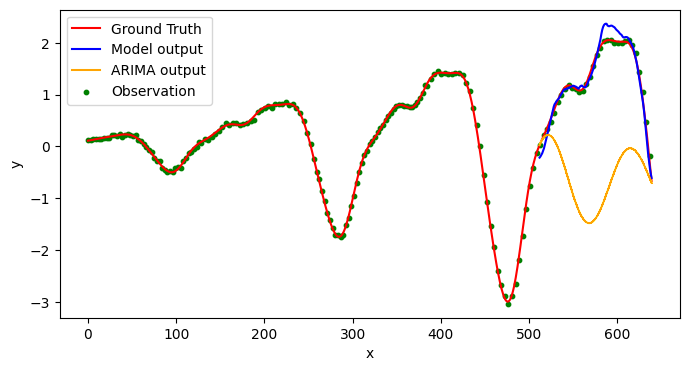
\includegraphics[width=\linewidth]{assets/validation1.png}
    \caption{Your caption here.}
    \label{fig:validation1}
\end{figure}
Looking at the plots of the predictions generated by our model on the validation set, we observed that the model performs well on data with high periodicity (see Figure~\ref{fig:validation1}). Since the functions and the parameters for the Gaussian process are sampled randomly, it is possible to encounter functions with less clear patterns (see Figure~\ref{fig:validation2}). These functions pose a challenge for the model, as it cannot anticipate their behavior in advance. This results in the model learning the average course of such functions. We postulate that this behavior negatively impacts the model's performance on functions where distinct patterns are present. It's therefore crucial to have checks in place to ensure that the model is only trained on data that exhibits clear patterns or aligns with the desired characteristics of the target task. This may help prevent the model from overfitting to noise or learning irrelevant trends.

 
\begin{figure}[h!]
    \centering
    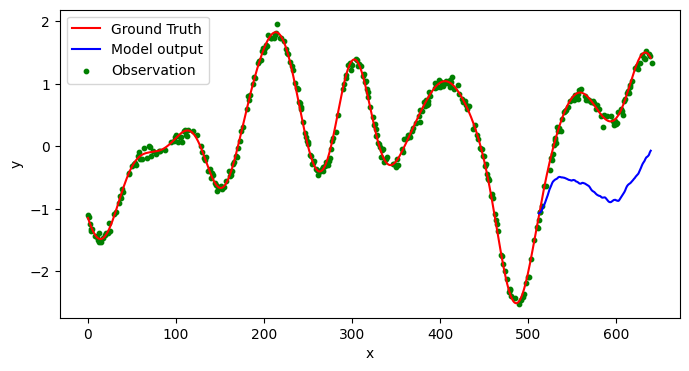
\includegraphics[width=\linewidth]{assets/validation2.png}
    \caption{Your caption here.}
    \label{fig:validation2}
\end{figure}

\subsection{Findings on ETTh1}
ETTh1 is a time series dataset containing data from various domains, such as oil temperature and electrical charge. We evaluate our model with a time horizon of 96, which corresponds to capturing 480 data points. These are split into $K=5$ windows, with the task being to predict the 5th window. 
The five windows are then shifted by one to the right and evaluated again.
The same procedure is applied for the time horizon of 192.
\begin{table}[h!]
    \centering
    \begin{tabular}{|c|c|c|c|c|}
    \hline
    \textbf{} & S & PE & PE + CSL & TimesFM \\ \hline 
    Validation   & 0.576             & 0.579             & 0.585             & -       \\ \hline
    ETTh1 - 96   & 0.966             & 0.968            & 0.928      &0.43*             \\ \hline
    ETTh1 - 192  & 1.0904            & 1.089            & 1.043            & 0.43*                     \\ \hline

\end{tabular}
    \caption{MAE results for three model variants and TimesFM on two datasets.\\
    \textit{*} TimesFM \cite{} only reports the average score over both time horizons. Additionally, they use only 4 datasets from ETTh1, which they do not disclose.
    }
    \label{tab:evaluation_results}
\end{table}
We evaluate our different model variants on the entire ETTh1 dataset in a zero-shot manner, meaning that we evaluate on all sub-datasets contained within ETTh1 and calculate the average performance.
Additionally, we compare our model to the one proposed by TimesFM \cite{}, using their accuracy score as a benchmark.
As shown in Table~\ref{tab:evaluation_results}, positional encoding does not appear to offer a significant benefit over the standard model. However, the PE + CSL approach provides slightly better performance. We also observe that the zero-shot performance of TimesFM on ETTh1-96 is much better than that of our current model. It is important to note, however, that TimesFM has been trained on a variety of data, both real-world and synthetic, and is approximately an order of magnitude larger in terms of parameter count.
We observe the same ordering of models for a horizon window of 192, where the PE + CSL version performs slightly better than the vanilla and PE versions.

\begin{figure}[h!]
    \centering
    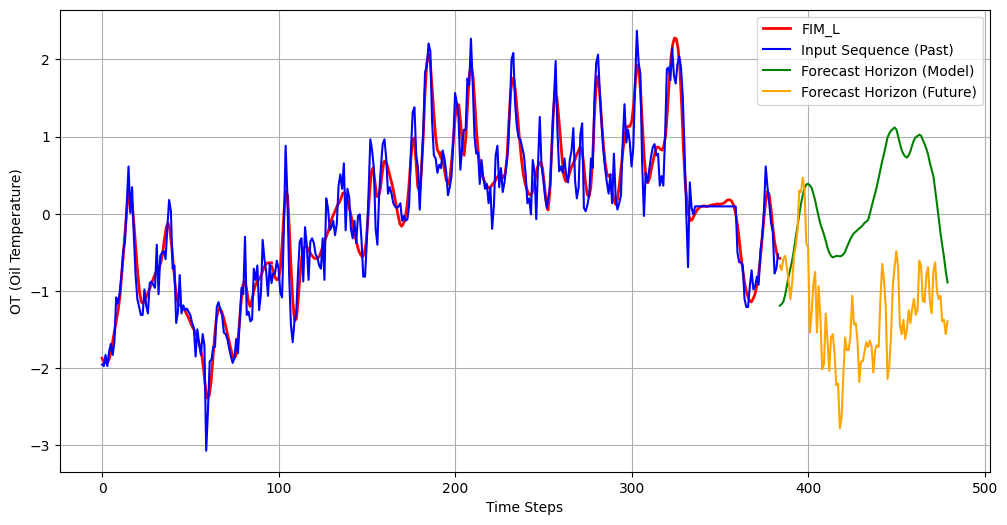
\includegraphics[width=\linewidth]{assets/etth128-fail.png}
    \caption{Example of good performance on the oil temperature dataset with $\text{horizon}=96$, using the PE + CSL model version.
    }
    \label{fig:etth96-success}
\end{figure}
Finally, we present two examples from the ETTh1 dataset using our model to showcase both well-performing and poorly-performing cases. In Figure~\ref{fig:etth96-success}, the model successfully predicts the horizon, as the data follows a very predictable pattern. However, in Figure~\ref{fig:etth96-fail}, we observe that the model struggles to accurately predict the horizon probably due to the lack of a very clear pattern in the data.


\begin{figure}[h!]
    \centering
    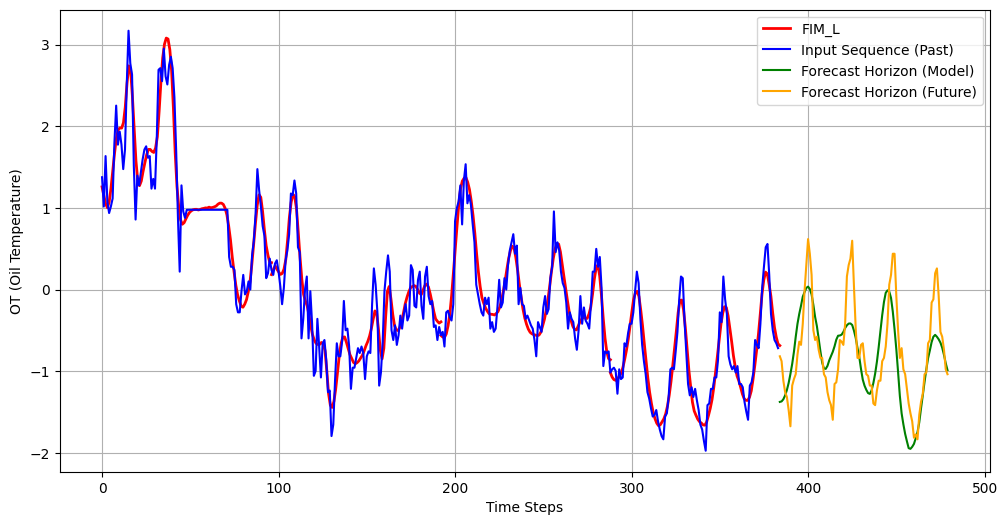
\includegraphics[width=\linewidth]{assets/etth128-success.png}
    \caption{Example of bad performance on the oil temperature dataset with $\text{horizon}=96$, using the PE + CSL model version.
    }\label{fig:etth96-fail}
\end{figure}
This suggests that our networks would likely benefit significantly from training on more diverse and real-world datasets, allowing them to learn patterns that are more subtle than those generated by a Gaussian process with a periodic kernel.

\section{Conclusion}

% In the unusual situation where you want a paper to appear in the
% references without citing it in the main text, use \nocite
\nocite{langley00}

\bibliography{example_paper}
\bibliographystyle{icml2025}


%%%%%%%%%%%%%%%%%%%%%%%%%%%%%%%%%%%%%%%%%%%%%%%%%%%%%%%%%%%%%%%%%%%%%%%%%%%%%%%
%%%%%%%%%%%%%%%%%%%%%%%%%%%%%%%%%%%%%%%%%%%%%%%%%%%%%%%%%%%%%%%%%%%%%%%%%%%%%%%
% APPENDIX
%%%%%%%%%%%%%%%%%%%%%%%%%%%%%%%%%%%%%%%%%%%%%%%%%%%%%%%%%%%%%%%%%%%%%%%%%%%%%%%
%%%%%%%%%%%%%%%%%%%%%%%%%%%%%%%%%%%%%%%%%%%%%%%%%%%%%%%%%%%%%%%%%%%%%%%%%%%%%%%
\newpage
\appendix
\onecolumn
\section{You \emph{can} have an appendix here.}

You can have as much text here as you want. The main body must be at most $8$ pages long.
For the final version, one more page can be added.
If you want, you can use an appendix like this one.  

The $\mathtt{\backslash onecolumn}$ command above can be kept in place if you prefer a one-column appendix, or can be removed if you prefer a two-column appendix.  Apart from this possible change, the style (font size, spacing, margins, page numbering, etc.) should be kept the same as the main body.
%%%%%%%%%%%%%%%%%%%%%%%%%%%%%%%%%%%%%%%%%%%%%%%%%%%%%%%%%%%%%%%%%%%%%%%%%%%%%%%
%%%%%%%%%%%%%%%%%%%%%%%%%%%%%%%%%%%%%%%%%%%%%%%%%%%%%%%%%%%%%%%%%%%%%%%%%%%%%%%


\end{document}


% This document was modified from the file originally made available by
% Pat Langley and Andrea Danyluk for ICML-2K. This version was created
% by Iain Murray in 2018, and modified by Alexandre Bouchard in
% 2019 and 2021 and by Csaba Szepesvari, Gang Niu and Sivan Sabato in 2022.
% Modified again in 2023 and 2024 by Sivan Sabato and Jonathan Scarlett.
% Previous contributors include Dan Roy, Lise Getoor and Tobias
% Scheffer, which was slightly modified from the 2010 version by
% Thorsten Joachims & Johannes Fuernkranz, slightly modified from the
% 2009 version by Kiri Wagstaff and Sam Roweis's 2008 version, which is
% slightly modified from Prasad Tadepalli's 2007 version which is a
% lightly changed version of the previous year's version by Andrew
% Moore, which was in turn edited from those of Kristian Kersting and
% Codrina Lauth. Alex Smola contributed to the algorithmic style files.
